\chapter{Thực nghiệm}
\label{Chapter4}

\section{Tập dữ liệu}

\setcounter{figure}{12}
\begin{figure}
	\centering
	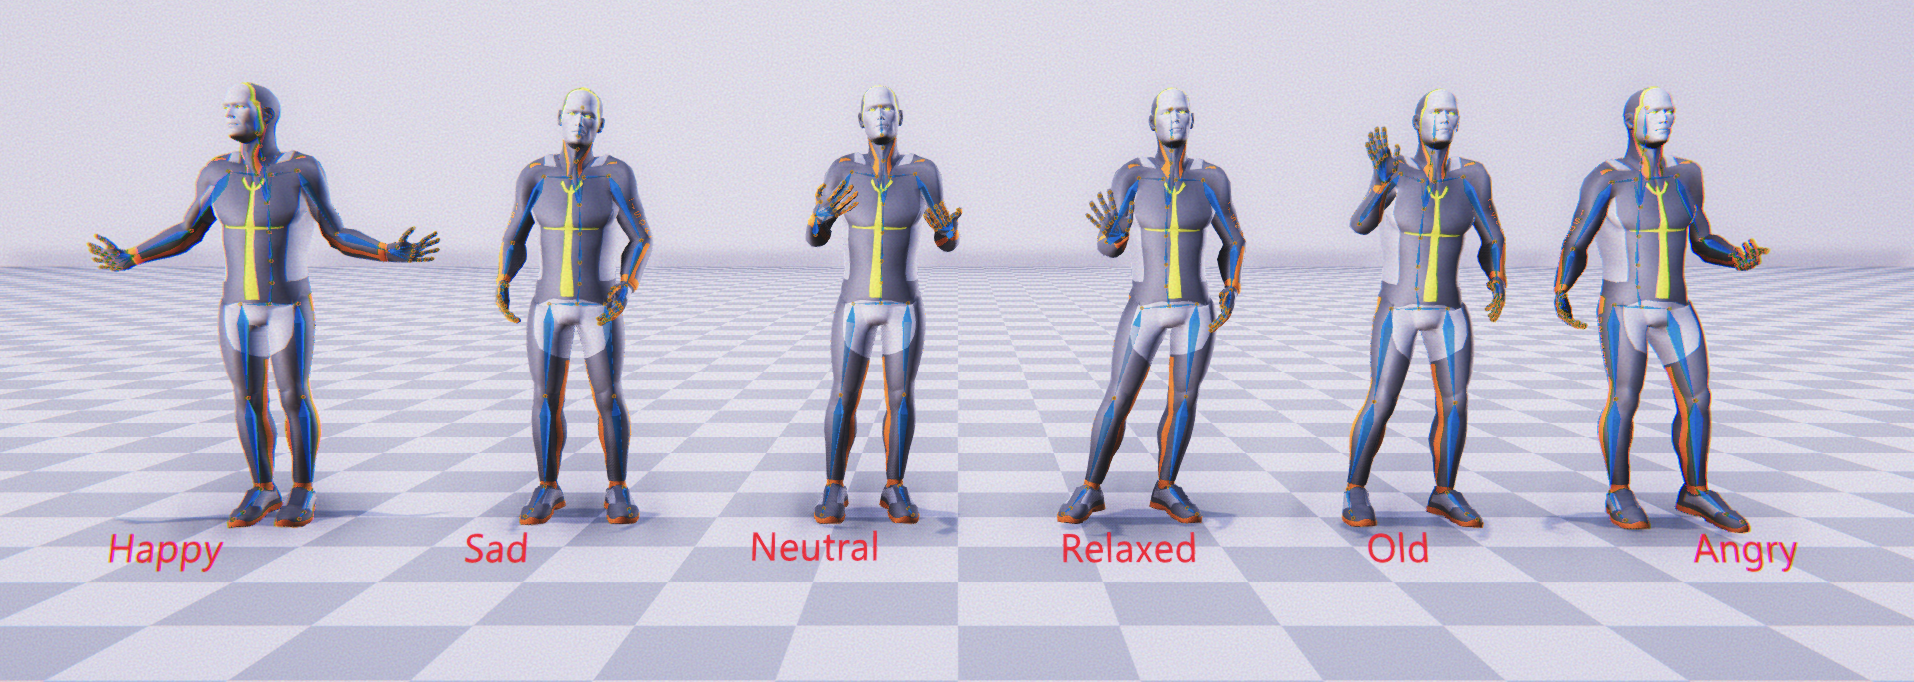
\includegraphics[width=\textwidth]{EmotionAnimation}
	\caption{Minh hoạ về 6 cử chỉ $\texttt{Happy}$, $\texttt{Sad}$, $\texttt{Neutral}$, $\texttt{Old}$, $\texttt{Relaxed}$ và $\texttt{Angry}$}
\end{figure}

Tập dữ liệu ZeroEGGS \cite{ghorbani2023zeroeggs} là một bộ dữ liệu motion capture được xây dựng để nghiên cứu và phát triển các mô hình tạo cử chỉ. Nó bao gồm 67 đoạn độc thoại do diễn viên motion capture nữ thực hiện, với tổng thời gian là 135 phút. Các đoạn hội thoại trong tập dữ liệu được biểu diễn với 6 cảm xúc khác nhau: $\texttt{Happy}$, $\texttt{Sad}$, $\texttt{Neutral}$, $\texttt{Old}$, $\texttt{Relaxed}$ và $\texttt{Angry}$, giúp mô phỏng nhiều trạng thái cảm xúc khác nhau trong cử chỉ và chuyển động cơ thể. ZeroEGGS cung cấp một nền tảng phong phú để nghiên cứu khả năng kết hợp giữa bài nói và cử chỉ động, phục vụ cho việc tạo ra các mô hình có thể điều chỉnh cử chỉ tương ứng với cảm xúc và ngữ nghĩa của văn bản.


\section{Quá trình huấn luyện}

Toàn bộ quá trình huấn luyện mô hình được thực hiện trong vòng 1 ngày với các tham số sau: số bước huấn luyện $T = 1000$, sử dụng GPU Nvidia 3090, và chia tập dữ liệu theo tỷ lệ $8:1:1$ cho các tập training, testing và validation. Learning rate được thiết lập là $3 \times 10^{-5}$, với batch size là 384 và tổng cộng 300,000 mẫu. Quá trình huấn luyện được triển khai trên mã nguồn chương trình có sẵn tại: \hyperlink{https://github.com/hmthanh/OHGesture}{hmthanh/OHGesture} .

\section{Phương pháp đánh giá}
\label{sec:evaluation}

Quá trình đánh giá được thực hiện qua hai độ đo chính là: Mean Opinion Scores (MOS) và Fréchet Inception Distance (FID).

\subsection{Mean Opinion Scores (MOS)}

Hiện tại, chưa có một độ đo chung cho bài toán sinh cử chỉ, đặc biệt là sinh cử chỉ từ âm thanh, vì vậy chúng tôi dựa vào đánh giá chủ quan của con người để thực hiện các đánh giá thực nghiệm. 
Tương tự như các phương pháp trước đây \cite{yoon2022genea}; \cite{kucherenko2021large}; các mô hình sinh cử chỉ điều khiển bằng giọng nói vẫn thiếu các chỉ số mục tiêu phản ánh một cách nhất quán với nhận thức chủ quan của con người  \cite{alexanderson2022listen}.
MOS được đo lường thông qua ba tiêu chí:

\begin{itemize}
	\item Human-likeness (Mức độ giống con người)
	\item Gesture-Speech Appropriateness (Sự phù hợp giữa cử chỉ và lời nói)
	\item Gesture-style Appropriateness (Sự phù hợp giữa phong cách cử chỉ)
\end{itemize}


\subsection{Fréchet Inception Distance (FID)}
FID đo sự tương đồng về phân phối giữa cử chỉ sinh ra $\mathbf{g}$ và cử chỉ thực tế $\mathbf{r}$. Công thức tính FID là:

\begin{equation}
	\text{FID} = \left\| \mu_r - \mu_g \right\|^2 + \operatorname{Tr}\left( \Sigma_r + \Sigma_g - 2 \sqrt{\Sigma_r \Sigma_g} \right)
\end{equation}

%\begin{itemize}
%	\item $\mu_r$ và $\Sigma_r$ là vector trung bình và ma trận hiệp phương sai của đặc trưng từ dữ liệu thực tế (real gestures).
%	\item $\mu_g$ và $\Sigma_g$ là vector trung bình và ma trận hiệp phương sai của đặc trưng từ cử chỉ tổng hợp (generated gestures).
%	\item $\|\mu_r - \mu_g\|^2$ là bình phương khoảng cách Euclidean giữa các vector trung bình.
%	\item $\text{Tr}\left( \Sigma_r + \Sigma_g - 2\sqrt{\Sigma_r \Sigma_g} \right)$ là trace của ma trận hiệp phương sai kết hợp, đo lường sự khác biệt giữa hai phân phối Gaussian.
%\end{itemize}

Trong đó:

\begin{itemize}
	\item $\mu$: Trung bình các đặc trưng của cử chỉ.
	\item $\Sigma$: Ma trận hiệp phương sai của đặc trưng.
	\item $\operatorname{Tr}$: Tổng đường chéo chính của ma trận hiệp phương sai.
	\item $\sqrt{\Sigma_r \Sigma_g}$: Sự tương đồng giữa các phân phối cử chỉ thực tế và cử chỉ sinh ra.
\end{itemize}

FID thấp cho thấy phân phối của cử chỉ sinh ra gần giống với cử chỉ thực tế, trong khi FID cao gợi ý sự khác biệt lớn, cho thấy chất lượng cử chỉ sinh ra kém hơn.



%\begin{itemize}
	%		\item \textbf{FID thấp}: Cho thấy phân phối của cử chỉ sinh ra rất gần với phân phối của cử chỉ thực tế, tức là cử chỉ tổng hợp trông tự nhiên hơn.
	%		\item \textbf{FID cao}: Gợi ý rằng các cử chỉ sinh ra khác biệt nhiều so với các cử chỉ thực tế, tức là chất lượng kém hơn.
	%	\end{itemize}
%	




% ngay cả với Fréchet gesture distance (FGD) \cite{yoon2022genea}, \cite{dabral2023mofusion}. Vì vậy, tất cả các điểm số thực nghiệm trong nghiên cứu này được thực hiện thông qua đánh giá chủ quan của con người. Chúng tôi đánh giá trên ba tiêu chí: độ giống con người, sự phù hợp giữa cử chỉ và giọng nói, và sự phù hợp giữa cử chỉ và phong cách. Các tiêu chí này được lấy từ đánh giá trong GENEA \cite{yoon2022genea}.


%Chúng tôi so sánh mô hình đề xuất của chúng tôi với StyleGestures \cite{alexanderson2020style}, Audio2Gestures \cite{li2021audio2gestures}, ExampleGestures \cite{ghorbani2023zeroeggs}.

\section{So sánh với các phương pháp hiện tại}
\label{sec:result}


Ở đây chúng tôi sử dụng lại kết quả đánh giá của mô hình baseline \textbf{DiffuseStyleGesture} \cite{yang2023diffusestylegesture} trong độ đo về  cảm nhận đánh giá của con người do lĩnh vực sinh cử chỉ vẫn còn rất mới, chi phí để ước lượng các mô hình còn lớn nên chúng tôi không thể đánh giá được mô hình OHGesture. Vì vậy các kết quả này chưa bao gồm thông tin kết qủa về mô hình \textbf{OHGesture} mà chúng tôi đề xuất.

\begin{figure}[htbp]
	\centering
	\begin{subfigure}[b]{0.3\textwidth}
		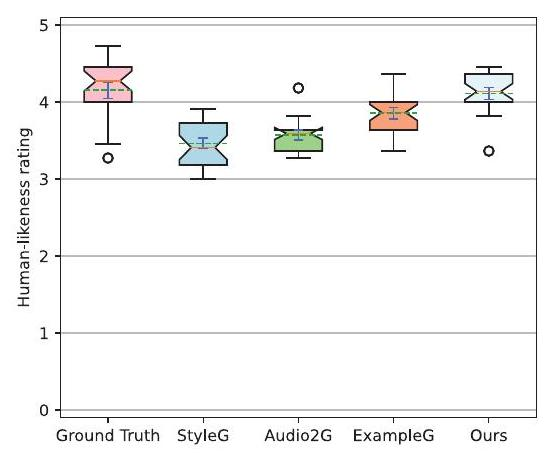
\includegraphics[width=\textwidth]{humanlike_score.jpg}
		\caption*{(a) Human-likeness}
	\end{subfigure}
	\hfill
	\begin{subfigure}[b]{0.3\textwidth}
		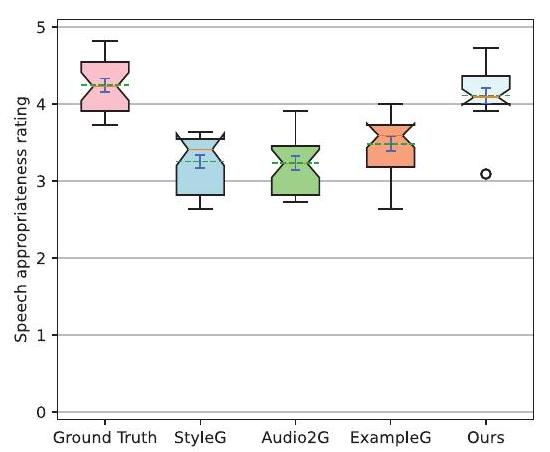
\includegraphics[width=\textwidth]{speech_score.jpg}
		\caption*{\small (b) Speech Appropriateness}
	\end{subfigure}
	\hfill
	\begin{subfigure}[b]{0.3\textwidth}
		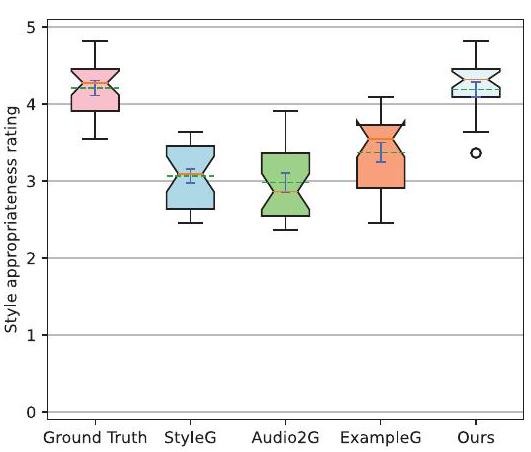
\includegraphics[width=\textwidth]{style_score.jpg}
		\caption*{(c) Style Appropriateness}
	\end{subfigure}
	
	%	    \caption[Biểu đồ hộp mô tả kết quả so sánh MOS]{Biểu đồ hộp mô tả kết quả so sánh MOS cho các mô hình khác nhau trong các chiều khác nhau. Hộp mở rộng từ phân vị thứ nhất thấp nhất (Q1) đến phân vị thứ ba lớn nhất (Q3) của dữ liệu. Đường đỏ chỉ là giữa. Các khe nhỏ biểu thị khoảng tin cậy $95\%$ (CI) xung quanh giữa. Khi CI nhỏ hơn Q1 hoặc lớn hơn Q3, khe mở rộng ra khỏi hộp, tạo ra một hình dáng "lật" độc đáo. Chúng tôi cũng đã đánh dấu giá trị trung bình và khoảng tin cậy $95\%$ của nó trong hình với đường nét đứt màu xanh lá cây và đường dọc màu xanh lam, tương ứng.}
	\label{fig:compare }
\end{figure}


Để hiểu hiệu suất thị giác thực tế của phương pháp của chúng tôi, chúng tôi tiến hành một nghiên cứu người dùng so sánh các cử chỉ được tạo ra từ phương pháp của chúng tôi và dữ liệu chụp chuyển động thực tế. Độ dài của các đoạn clip đánh giá dao động từ 11 đến 51 giây, với độ dài trung bình là 31.6 giây, dài hơn so với các đoạn trong đánh giá GENEA \cite{yoon2022genea} (8-10 giây), vì thời gian dài hơn có thể tạo ra kết quả rõ ràng và thuyết phục hơn \cite{yang2022reprgesture}. Người tham gia đánh giá trên thang điểm từ 5 đến 1, với các nhãn từ $\texttt{excellent}$,  $\texttt{good}$, $\texttt{fair}$, $\texttt{poor}$, đến $\texttt{bad}$. 


\begin{table}[!t]
	\centering
		\begin{tabular}{lcc}
			\hline
			\multicolumn{1}{c}{Name} &
			\begin{tabular}[c]{@{}c@{}}Human\\ likeness \end{tabular}$\uparrow$ &
			\begin{tabular}[c]{@{}c@{}}Gesture-speech\\ appropriateness\end{tabular}$\uparrow$ \\ \hline
			Ground Truth          & 4.15 $\pm$ 0.11          & 4.25 $\pm$ 0.09          \\
			Ours                  & \textbf{4.11 $\pm$ 0.08} & \textbf{4.11 $\pm$ 0.10} \\
			\quad$-$ WavLM             & 4.05 $\pm$ 0.10          & 3.91 $\pm$ 0.11          \\
			\quad$-$ Cross-local attention   & 3.76 $\pm$ 0.09          & 3.51 $\pm$ 0.15          \\
			\quad$-$ Self-attention    & 3.55 $\pm$ 0.13          & 3.08 $\pm$ 0.10          \\
			% \begin{tabular}[c]{@{}c@{}}$-$ attention (GRU based) \\ (GRU based)\end{tabular} &
			\quad$-$ Attention + GRU&
			3.10 $\pm$ 0.11 &
			2.98 $\pm$ 0.14 \\
			\quad$+$ Forward attention & 3.75 $\pm$ 0.15          & 3.23 $\pm$ 0.24          \\
			\hline
		\end{tabular}s
	\caption{Kết quả của các nghiên cứu loại bỏ (Ablation studies). "$-$" chỉ các mô-đun không được sử dụng và "$+$" chỉ các mô-đun bổ sung. Chữ in đậm chỉ ra chỉ số tốt nhất.}
	\label{Ab}
\end{table}


\section{Xây dựng và tiêu chuẩn hoá hệ thống đánh giá kết quả sinh cử chỉ}

Hiện nay các mô hình sinh (gesture generation) cử chỉ được quan tâm nghiên cứu với rất nhiều mô hình khác nhau, tuy nhiên do không có độ đo chung, vì các độ đo truyền thống như FID (Fréchet Inception Distance) hay IS (Inception Score),.. không thể hiện được hết các tính chất Giống người (Human-likeness), tính phù hợp với giọng nói (Speech Appropriateness), và tính phù hợp với phong cách (Style Appropriateness) của cử chỉ. Các mô hình cũng được thực hiện và huấn luyện trên một tập dữ liệu khác nhau, vì vậy rất khó để biết được mô hình nào đã đạt kết quả tốt hơn, và mô hình nào là state-of-the-art, từ đó khó có thể đạt được sự tiến bộ trong lĩnh vực sinh cử chỉ. Việc thiếu tiêu chuẩn chung để đánh giá trong cộng đồng nghiên cứu khiến chúng tôi mong muốn xây dựng một hệ thống xếp hạng trực tuyến \cite{nagy2024towards} \hyperlink{https://genea-workshop.github.io/leaderboard/}{GENEA Leaderboard}, là một bảng xếp hạng các mô hình sinh cử chỉ. Chúng tôi thu thập và xử lý một tập dữ liệu cử chỉ từ nhiều ngôn ngữ và từ nhiều tập dữ liệu khác nhau và tiêu chuẩn hoá để tạo ra một tập dữ liệu duy nhất.  Sau đó, chúng tôi sẽ mời các tác giả của các mô hình để học và dự đoán trên tập dữ liệu đã được tiêu chuẩn hoá, sau khi có kết quả sinh cử chỉ, chúng tôi sẽ thuê những người tham gia nghiên cứu trên Prolific để đánh giá và xếp hạng kết quả sinh cử chỉ của các mô hình. Hiện tại chúng tôi đang xây dựng hệ thống trực tuyến \hyperlink{https://github.com/hemvip/hemvip.github.io}{hemvip/hemvip.github.io} với mục tiêu đánh giá kết quả sinh của cử chỉ thông qua việc thuê các người tham gia đánh giá kết quả thông qua Prolific. Chúng tôi sẽ bổ sung các đánh giá về mô hình OHGesture dựa trên các điểm số trên.

Thông qua hệ thống đánh giá này, nghiên cứu kỳ vọng sẽ thiết lập một tiêu chuẩn chung, từ đó tạo động lực cho sự tiến bộ trong lĩnh vực sinh cử chỉ.

%Chi tiết về nghiên cứu người dùng có thể được tìm thấy trong tư liệu bổ sung.

%Điểm số ý kiến trung bình (MOS) về độ giống con người, sự phù hợp giữa cử chỉ và giọng nói, và sự phù hợp giữa cử chỉ và phong cách được báo cáo trong \ref{fig}. 
%Nếu các góc của hai hộp không chồng lên nhau, điều này chứng tỏ rằng các phân phối khác biệt đáng kể \cite{mcgill1978variations}. Phương pháp của chúng tôi vượt trội so với các phương pháp tiên tiến được so sánh trong cả ba chiều đánh giá, và thậm chí tạo ra các kết quả cạnh tranh với dữ liệu thực tế. Phản hồi từ người tham gia cho thấy cử chỉ do phương pháp của chúng tôi tạo ra "có ý nghĩa ngữ nghĩa hơn", "tự nhiên hơn", và "phù hợp với phong cách", mặc dù có một số vấn đề về "chuyển động trượt chân" so với Dữ liệu Thực. Tuy nhiên, đây là một vấn đề phổ biến đối với các hệ thống tạo ra chuyển động không dựa trên vật lý và có thể được giải quyết thông qua xử lý sau \cite{ghorbani2023zeroeggs}, \cite{luvizon2023scene}.

%Hiện tại chưa có một độ đo chung cho bài toán sinh cử chỉ, đặc biệt là sinh cử chỉ từ âm thanh, vì vậy chúng tôi 
%các cử chỉ điều khiển bằng giọng nói thiếu các chỉ số mục tiêu phản ánh một cách nhất quán với nhận thức chủ quan của con người \cite{yoon2022genea}; \cite{kucherenko2021large}; \cite{alexanderson2022listen}, ngay cả với Fréchet gesture distance (FGD) \cite{yoon2022genea}, \cite{dabral2023mofusion}, do đó tất cả các điểm số thực nghiệm của chúng tôi được thực hiện thông qua đánh giá chủ quan của con người. Chúng tôi thực hiện đánh giá trên ba chiều. Hai chiều đầu tiên theo đánh giá trong GENEA \cite{yoon2022genea}, bao gồm đánh giá về độ giống con người và sự phù hợp giữa cử chỉ và giọng nói. Chiều thứ ba là sự phù hợp giữa cử chỉ và phong cách.
%
%Nghiên cứu Người Dùng. Để hiểu về hiệu suất thị giác thực tế của phương pháp của chúng tôi, chúng tôi tiến hành một nghiên cứu người dùng giữa các trình tự cử chỉ được tạo ra bởi mỗi phương pháp được so sánh và dữ liệu chụp chuyển động thực. Độ dài của các đoạn clip được đánh giá dao động từ 11 đến 51 giây, với độ dài trung bình là 31.6 giây. Lưu ý rằng các cử chỉ clip được sử dụng cho đánh giá chủ quan ở đây dài hơn so với đánh giá GENEA \cite{yoon2022genea} (8-10 giây), vì một khoảng thời gian dài có thể tạo ra kết quả phù hợp rõ ràng và thuyết phục hơn \cite{yang2022reprgesture}. Người tham gia đánh giá trên một khoảng điểm từ 5 đến 1, với các nhãn (tốt nhất đến tệ nhất) là "tuyệt vời," "tốt," "công bằng," "kém," và "tệ." Thêm chi tiết về nghiên cứu người dùng được hiển thị trong tư liệu bổ sung.
%
%
%
%
%
%
%Điểm số ý kiến trung bình (MOS) về độ giống con người, phù hợp giọng nói và phù hợp phong cách được báo cáo trong \ref{fig:mosscore}. Nếu các góc của hai hộp không chồng lên nhau, chúng ta có thể coi đây là bằng chứng mạnh mẽ rằng các phân phối khác nhau đáng kể \cite{mcgill1978variations}. Phương pháp của chúng tôi vượt trội đáng kể so với các phương pháp tiên tiến được so sánh với độ giống con người, phù hợp giữa cử chỉ và giọng nói, cũng như phù hợp giữa cử chỉ và phong cách, và thậm chí tạo ra các kết quả cạnh tranh với dữ liệu thực tế ở cả ba chiều. Theo phản hồi từ người tham gia, cử chỉ được tạo ra bởi chúng tôi "có ý nghĩa ngữ nghĩa hơn", "tự nhiên hơn," và "phù hợp với phong cách," trong khi phương pháp của chúng tôi có "chuyển động trượt chân" so với Dữ liệu Thực. Tuy nhiên, đây là một vấn đề phổ biến đối với các hệ thống tạo ra chuyển động không dựa trên vật lý và có thể được giải quyết thông qua xử lý sau \cite{ghorbani2023zeroeggs}, \cite{luvizon2023scene}.

%\begin{table}[t]
%	\centering
%	\caption{Impact of the positional encoding block.}
%	\label{tab:pos_enc}
%	
%	\newcolumntype{Y}{>{\raggedleft\arraybackslash}X}
%	\newcolumntype{Z}{>{\centering\arraybackslash}X}
%%	\begin{tabularx}{\linewidth}{XlYY}
%	
%%		
%	
%%		\bottomrule
%%		\begin{tabularx}{\linewidth}{XlYY}
%%		\toprule
%%		Dataset & System & FGD $\downarrow$ & PMB ($\%$) $\uparrow$ \\
%%		\toprule
%%		\multirow{2}{*}{TED} & Without positional encoding & 2.19 & 88.13 \\
%%		& With positional encoding & $\bm{2.04}$ & $\bm{89.52}$ \\
%%		\bottomrule
%%		\end{tabularx}
%
%
%
%
%% \begin{tabularx}{\linewidth}{XlYY}
%%	\toprule
%%	Dataset & System & FGD $\downarrow$ & PMB ($\%$) $\uparrow$ \\
%%	\toprule
%%	\multirow{2}{*}{TED} & encoding & 2.19 & 88.13 \\
%%	& With positional encoding & $2.04$ & $89.52$ \\
%%	\bottomrule
%%\end{tabularx}
%
%
%
%%		\multirow{2}*{Trinity} & Without positional encoding & 11.15 & 89.98 \\
%%				& With positional encoding & $\bm{10.78}$ & $\bm{91.36}$ \\
%%\hline
%%This is a long entry that will automatically adjust its width. & Short text & Another long entry that will also adjust its width. \\
%%\hline
%%More text & Another short entry & Yet another long entry to demonstrate text wrapping and width adjustment. \\
%%\hline
%
%\end{table}



% \section{Đánh Giá}
% \label{sec:experiments}
 % Khả năng Kiểm soát Cử chỉ

%\subsection{Khả năng kiểm soát cử chỉ}
%\label{subsec:stylecontrol}

%Giả sử rằng âm thanh trung tính không ảnh hưởng đến phong cách của cử chỉ, chúng ta có thể tạo ra các cử chỉ được phong cách hóa với một bài nói trung tính bằng cách đặt $\gamma=1$ và $e$ trong \ref{eq:denoise}. Chúng tôi chọn hai đoạn hội thoại trong tập kiểm thử với âm thanh trung tính để tạo ra sáu cử chỉ được phong cách hóa tương ứng. \ref{fig:emotiondataset} minh họa cử chỉ được tạo ra $\hat{\mathbf{x}}_{t}$ của các phong cách đầu vào $s$ khác nhau với cùng một âm thanh trung tính được thị giác hóa bằng phương pháp tSNE.
%
%\begin{figure}
%    \centering
%    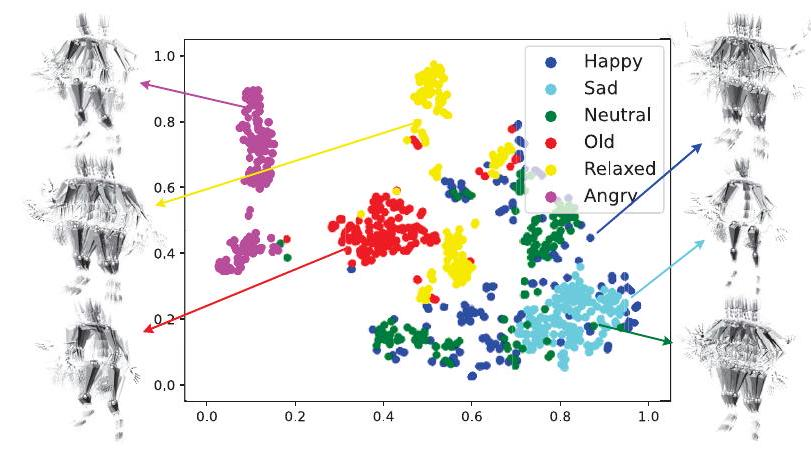
\includegraphics[width=0.7\linewidth]{images/emotion_dataset.jpg}
%    \caption[Biểu đồ tSNE với các phong cách khác nhau]{Hiển thị tSNE của các cử chỉ với các phong cách khác nhau và bản đồ bóng của cử chỉ xương cơ với phong cách tương ứng. Ví dụ, với cử chỉ 'Old', hông và đầu gối của nó uốn cong hơn, và tay của nó cơ bản nằm ở đầu gối hoặc hông.}
%    \label{fig:emotiondataset}
%\end{figure}
%
%Chúng tôi cũng vẽ biểu đồ xương cơ được tạo ra bởi phong cách tương ứng trong hình, và có thể thấy rằng đối với phong cách 'Old', hông và đầu gối của nó uốn cong hơn, và tay của nó cơ bản nằm ở đầu gối hoặc hông; với phong cách 'Sad', đầu của nó đang nghiêng và tay nó ở một vị trí thấp hơn; với phong cách 'Relax', hông của nó đang chuyển lên phía trước và tư thế đứng của nó là thoải mái; với phong cách 'Angry', tay của nó di chuyển lên và xuống nhanh chóng. Lưu ý rằng mặc dù sự khác biệt giữa cử chỉ phong cách 'trung tính' và 'Happy' vẫn khá rõ ràng trong việc thị giác hóa phong cách của xương cơ, tức là với phong cách 'Happy', vị trí tay của nó là cao hơn và biên độ của nó lớn hơn, tuy nhiên tSNE của chúng gần như kết hợp với nhau. Trong phân tích của chúng tôi, điều này xảy ra vì bài nói trung tính gọi là vẫn chứa thông tin như cảm xúc và ngữ nghĩa mà có trong các đặc trưng WavLM. Sự cân bằng giữa phong cách từ âm thanh $\mathbf{a}$ và từ phong cách $\mathbf{e}$ có thể được kiểm soát thêm bằng cách chỉnh sửa cường độ phong cách $\gamma$.
%
%Giả sử rằng âm thanh Neutral không ảnh hưởng đến cảm xúc của cử chỉ, chúng ta có thể tạo ra các cử chỉ được điều chỉnh theo cảm xúc với một bài nói Neutral bằng cách đặt $\gamma=1$ và $e$ trong \ref{eq:denoise}. Chúng tôi chọn hai đoạn hội thoại trong tập kiểm thử với âm thanh trung tính để tạo ra sáu cử chỉ được điều chỉnh cảm xúc tương ứng. Hình \ref{fig:emotiondataset} minh họa cử chỉ được tạo ra $\hat{\mathbf{x}}_{t}$ cho các cảm xúc đầu vào $s$ khác nhau với cùng một âm thanh trung tính, được thị giác hóa bằng phương pháp t-SNE.
%
%\begin{figure}
%	\centering
%	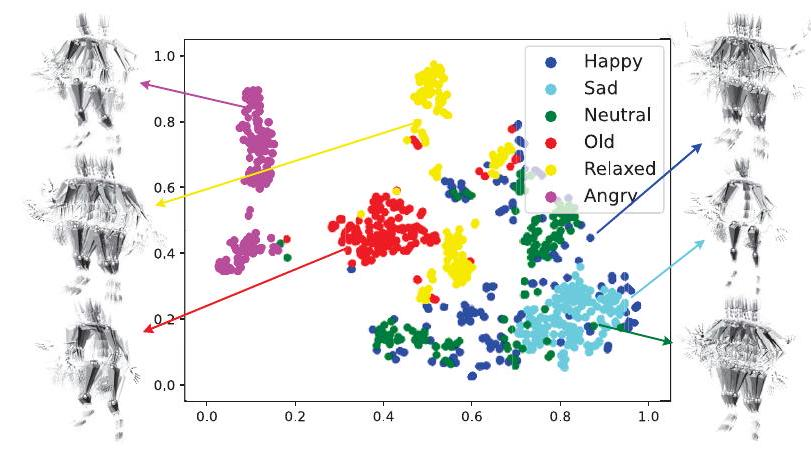
\includegraphics[width=0.7\linewidth]{images/emotion_dataset.jpg}
%	\caption[Biểu đồ t-SNE với các cảm xúc khác nhau]{Hiển thị t-SNE của các cử chỉ với các cảm xúc khác nhau và bản đồ bóng của cử chỉ xương cơ với cảm xúc tương ứng. Ví dụ, với cử chỉ 'Old', hông và đầu gối của nó uốn cong hơn, và tay của nó cơ bản nằm ở gần đầu gối hoặc hông.}
%	\label{fig:emotiondataset}
%\end{figure}
%
%Chúng tôi cũng biểu diễn các cử chỉ khung xương tương ứng với từng cảm xúc trong hình và nhận thấy rằng đối với cảm xúc 'Old', hông và đầu gối có độ uốn cong lớn hơn, và tay chủ yếu nằm ở đầu gối hoặc hông; với cảm xúc 'Sad', đầu nghiêng và tay ở vị trí thấp hơn; với cảm xúc 'Relaxed', hông hơi hướng về phía trước với tư thế đứng thoải mái; với cảm xúc 'Angry', tay chuyển động nhanh chóng lên xuống. Lưu ý rằng mặc dù sự khác biệt giữa cử chỉ với cảm xúc 'Neutral' và 'Happy' vẫn rõ ràng khi thị giác hóa khung xương, cụ thể là với cảm xúc 'Happy', tay ở vị trí cao hơn và biên độ lớn hơn, nhưng các điểm t-SNE của chúng lại gần nhau. Trong phân tích của chúng tôi, điều này là do bài nói trung tính vẫn chứa thông tin về cảm xúc và ngữ nghĩa từ các đặc trưng của WavLM. Sự cân bằng giữa cảm xúc từ âm thanh $\mathbf{a}$ và từ điều chỉnh cảm xúc $\mathbf{e}$ có thể được kiểm soát thêm thông qua việc điều chỉnh cường độ cảm xúc $\gamma$.



%\subsection{Khả năng điều chỉnh cảm xúc của cử chỉ}
%
%
%\begin{figure}
%	\centering
%	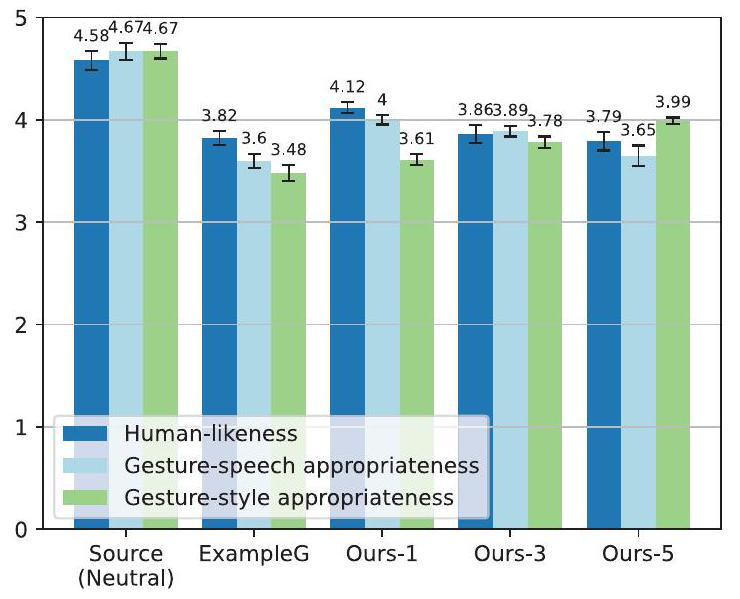
\includegraphics[width=0.7\linewidth]{images/mos_score.jpg}
%	\label{fig:mosscore}
%	\caption{Kết quả trung bình của MOS}
%	
%	%    \caption[Kết quả trung bình của MOS]{Kết quả trung bình của MOS với khoảng tin cậy $95\%$ cho ba chiều. 'Ours-$\gamma$' chỉ ra cường độ kiểm soát phong cách $\gamma$ của mô hình của chúng tôi. Mô hình của chúng tôi vượt trội đáng kể so với ExampleGesture tổng thể và có thể chỉnh sửa cường độ của các phong cách. Tham số $\gamma$ tăng và hai điểm số còn lại sẽ giảm một cách hợp lý.}
%	
%	\vspace{-10pt}
%\end{figure}

%Trong nghiên cứu này, chúng tôi điều chỉnh cường độ cảm xúc của cử chỉ thông qua tham số $\gamma$, với các giá trị $\gamma=1$ và $\gamma=3$ cho cảm xúc 'Happy' và 'Old'. Khi $\gamma=3$, cảm xúc 'Happy' tạo ra cử chỉ mạnh mẽ với chuyển động tay và cơ thể rõ rệt, trong khi 'Old' thể hiện cử chỉ ít năng động hơn, với hông ít uốn cong và tay ít được nâng lên. Các giá trị $\gamma$ khác cho phép điều chỉnh cường độ cảm xúc, giúp tạo ra cử chỉ tương ứng với các cảm xúc chuyển tiếp giữa 'Happy' và 'Old'. Các thử nghiệm cho thấy rằng việc tăng $\gamma$ giúp tạo ra cử chỉ phù hợp với cảm xúc mong muốn, ngay cả khi chúng không có trong dữ liệu huấn luyện. 
%Một nghiên cứu người dùng cho thấy mô hình của chúng tôi vượt trội so với ExampleGesture trong việc điều chỉnh cường độ cảm xúc và tạo ra cử chỉ tự nhiên và phù hợp với ngôn ngữ.
%
%Để phân tích chi tiết hơn mối quan hệ giữa cường độ cảm xúc và cảm xúc mà bài nói ngụ ý, chúng tôi lựa chọn hai cảm xúc là 'Happy' và 'Old' và thiết lập $\gamma=1$ và $3$ trong \ref{eq:denoise}. Để so sánh kết quả, chúng tôi cũng thiết lập $\gamma=0.5$ trong \ref{eq:denoise} để nội suy giữa các cảm xúc khác nhau. Các tham số còn lại được giữ nguyên, và chúng tôi biểu diễn cử chỉ được tạo ra trong 12 giây với FPS $=1$.
%
%Có thể quan sát thấy rằng khi sử dụng cảm xúc 'Happy' với $\gamma=3$, chuyển động cơ thể và cử động tay đều đạt cường độ cao nhất, và vị trí tay được nâng cao nhất; ngược lại, khi sử dụng cảm xúc 'Old' với $\gamma=3$, hông có độ uốn cong lớn nhất, tay ít được nâng lên, và chuỗi chuyển động nhìn chung có ít thay đổi. Đối với ba kết quả còn lại, cường độ cảm xúc nằm giữa hai trường hợp này, với cảm xúc dần chuyển từ Happy sang Old. Kiến trúc mô hình của chúng tôi giúp cử chỉ và bài nói kết hợp với nhau hài hòa hơn, dù hai cảm xúc không hoàn toàn giống nhau. Lưu ý rằng khi sử dụng cảm xúc 'Happy' và 'Old' với $\gamma=0.5$, kết quả gần giống như khi sử dụng cảm xúc 'Happy' với $\gamma=1$, trong khi cảm xúc 'Old' khó nhận ra. Quan sát này khẳng định kết luận trước đó rằng cảm xúc 'Happy' đã được thể hiện trong bài nói 'Neutral' dùng để kiểm thử. Điều này cho thấy, chẳng hạn, trong các thử nghiệm của chúng tôi, nếu muốn điều chỉnh bài nói 'Happy' để tạo ra cử chỉ 'Sad', $\gamma=1$ có thể không hiệu quả do mô hình có xu hướng học cảm xúc Happy từ bài nói. Do sự tương quan giữa cảm xúc của bài nói và cảm xúc của cử chỉ, việc tăng giá trị $\gamma$ có thể giúp điều chỉnh cảm xúc tốt hơn, cho phép tạo ra các cử chỉ không có trong tập dữ liệu gốc (ví dụ: cử chỉ cho bài nói 'Happy' nhưng có cảm xúc 'Sad') thông qua việc điều chỉnh cường độ cảm xúc.
%
%Hơn nữa, để tìm hiểu mối quan hệ giữa cường độ cảm xúc với độ giống con người (human-likeness) và sự phù hợp với ngôn ngữ, chúng tôi đã tiến hành một nghiên cứu người dùng. Để tránh ảnh hưởng của cảm xúc trong ngôn ngữ nói đến đánh giá của người tham gia, tương tự như trước, chúng tôi chỉ điều chỉnh cường độ cảm xúc cho một bài nói Neutral và yêu cầu người tham gia đánh giá theo ba tiêu chí đặc trưng trước đó. ExampleGesture \cite{ghorbani2023zeroeggs} cũng cho phép kiểm soát việc tạo ra các cảm xúc khác nhau từ cùng một bài nói, vì vậy chúng tôi chọn nó làm mô hình tham chiếu. Do các cử chỉ được tạo ra ở đây không tồn tại trong tập dữ liệu, bài nói Neutral với cảm xúc trung tính được sử dụng làm tham chiếu.

%
%\subsection{Khả năng chỉnh sửa Phong cách của cử chỉ}
%
%Để phân tích sâu hơn mối quan hệ giữa cường độ phong cách và phong cách được ngụ ý bởi bài nói, chúng tôi chọn phong cách 'Happy' và phong cách 'Old' và đặt $\gamma=1$ và 3 trong \ref{eq:denoise}. Ngoài ra, để so sánh kết quả, chúng tôi đặt $\gamma=0.5$ trong \ref{eq:denoise}, để nội suy giữa các phong cách khác nhau. Các tham số khác không thay đổi, và chúng tôi vẽ kết quả tạo ra cử chỉ trong 12 giây, với FPS $=1$.
%%như thể hiện trong 
%%\ref{fig:stylesample}.
%
%
%%Như thấy trong
%% \ref{fig:stylesample}, 
% Chúng ta có thể thấy rằng khi chúng ta sử dụng phong cách 'Happy' với $\gamma=3$, cả quá trình xoay cơ thể và chuyển động tay đều lớn nhất, và vị trí tay của nó là cao nhất; ngược lại, khi chúng ta sử dụng phong cách 'Old' với $\gamma=3$, hông của nó uốn cong nhất, tay hầu như không được nâng lên, và không có nhiều sự thay đổi trong toàn bộ chuỗi chuyển động; còn đối với ba kết quả khác, cường độ phong cách của chúng ở giữa hai trường hợp trên, và phong cách dần thay đổi từ vui vẻ đến già từ trên xuống dưới. Do kiến trúc mô hình của chúng tôi, cử chỉ và bài nói được tạo ra phù hợp hơn, mặc dù các phong cách này không giống nhau. Lưu ý rằng khi chúng ta sử dụng phong cách 'Happy' và 'Old' với $\gamma=0.5$, kết quả gần với việc sử dụng phong cách 'Happy' với $\gamma=1$, trong khi phong cách 'Old' gần như không thể cảm nhận được. Quan sát này tiếp tục xác nhận phát hiện trước đó rằng phong cách 'Happy' được nhúng trong bài nói 'trung tính' được sử dụng để kiểm thử. Phát hiện này hữu ích, ví dụ, chúng tôi đã phát hiện trong các thử nghiệm của mình rằng nếu chúng ta muốn kiểm soát bài nói 'Happy' để tạo ra cử chỉ 'Sad', $\gamma=1$ cơ bản là không hiệu quả vì mô hình có thể học được phong cách vui vẻ từ bài nói. Vì có sự liên kết giữa phong cách của bài nói và phong cách của cử chỉ, việc đặt $\gamma$ lớn hơn có thể chỉnh sửa phong cách tốt hơn. Do đó, chúng ta có thể tạo ra các cử chỉ không tồn tại trong tập dữ liệu gốc (ví dụ, cử chỉ cho bài nói 'Happy' nhưng có phong cách 'Sad') thông qua cường độ phong cách.
%
%
%% Nghiên cứu Người dùng. 
%Hơn nữa, chúng tôi muốn khám phá mối quan hệ giữa cường độ phong cách và độ giống con người cũng như sự phù hợp với ngôn ngữ, nên chúng tôi đã tiến hành một nghiên cứu người dùng. Để tránh phong cách trong ngôn ngữ nói ảnh hưởng đến việc đánh giá của người tham gia, giống như trước đó, chúng tôi chỉ kiểm soát cường độ của các phong cách cho một bài nói trung tính và sau đó yêu cầu người tham gia đánh giá ba chiều đặc trưng trước đó. ExampleGesture \cite{ghorbani2023zeroeggs} cũng có thể kiểm soát việc tạo ra các phong cách khác nhau của các cử chỉ từ cùng một bài nói. Vì vậy, chúng tôi chọn nó làm mô hình tham chiếu. Vì các cử chỉ được tạo ra ở đây không tồn tại trong tập dữ liệu, bài nói trung tính với phong cách trung tính được sử dụng làm tham chiếu. 
%

%Kết quả được thể hiện trong hình \ref{fig:mosscore}.

%\begin{figure}
%    \centering
%    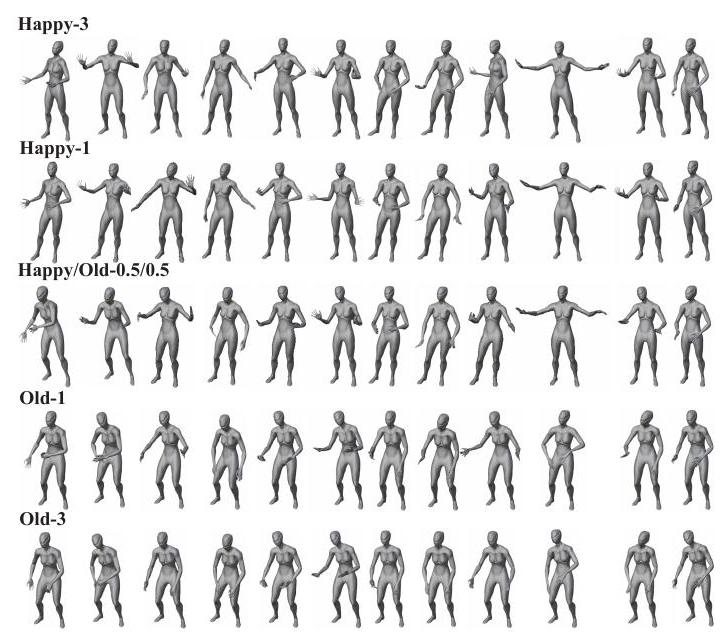
\includegraphics[width=0.6\linewidth]{images/style_sample.jpg}
%    \caption[Chỉnh sửa phong cách và nội suy]{\small Chỉnh sửa phong cách và nội suy. Từ trên xuống dưới, cơ thể xoắn và chuyển động tay dần giảm và vị trí tay trở nên thấp hơn. Mặc dù có sự thay đổi về phong cách, các cử chỉ được tạo ra vẫn khớp tốt với bài nói trong các phong cách khác nhau}
%    \label{fig:stylesample}
%\end{figure}


% % Hình 6: 



%Kết quả cho thấy rằng mô hình của chúng tôi tương tự như ExampleGesture về mặt phù hợp giữa phong cách cử chỉ của kết quả ở $\gamma=1$, và độ giống con người cũng như sự phù hợp với ngôn ngữ của chúng tôi vượt quá ExampleGesture. Trong khi đó, phong cách trở nên đáng kể hợp lý hơn khi $\gamma$ tăng, nhưng điểm của hai chiều khác giảm. Điều này cũng là hiển nhiên, tức là nếu cường độ của phong cách 'Old' quá cao, tay ít được nâng lên và toàn bộ chuỗi chuyển động có biên độ nhỏ, vì vậy nó trông ít giống con người hơn và ít phù hợp với ngôn ngữ nói. Chúng tôi cũng thấy rằng kết quả của việc tạo ra kiểm soát phong cách (\ref{fig:mosscore}) đã giảm so với kết quả của việc trực tiếp tạo ra phong cách tương ứng với ngôn ngữ nói (\ref{fig:mosscore}). Chúng tôi tin rằng việc kiểm soát một phong cách nói để tạo ra một phong cách của cử chỉ khác là một nhiệm vụ "khó khăn và xung đột" bởi vì phong cách nói và phong cách của cử chỉ vẫn liên quan và kết hợp với nhau.

% \subsection{Khả năng tạo ra các cử chỉ đa dạng}

% \begin{figure}
%     \centering
%     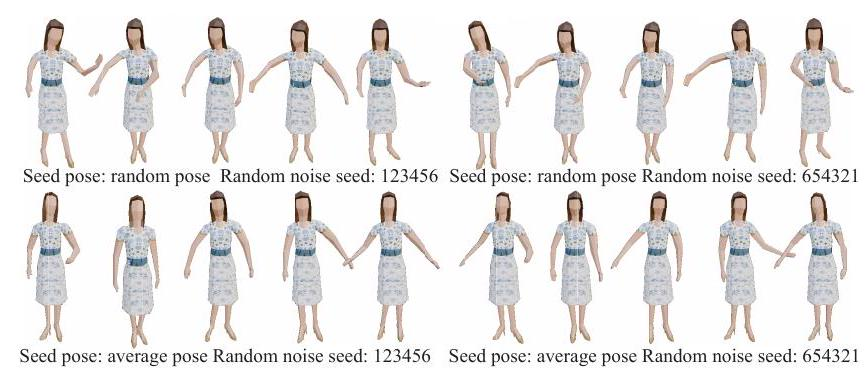
\includegraphics[width=\linewidth]{images/random_gesture_result.jpg}
%     \caption[Sự đa dạng của các cử chỉ]{Sự đa dạng của các cử chỉ. Mọi người thực hiện các cử chỉ đồng thoại khác nhau ở những thời điểm khác nhau trong các trạng thái khác nhau. Giống như con người thực tế, đối với cùng một bài nói, phương pháp của chúng tôi có khả năng tạo ra các cử chỉ khác nhau với hạt gieo khác nhau hoặc với cử chỉ nhiễu khác nhau}
%     \label{fig:randomgestureresult}
% \end{figure}


% \begin{center}
% \begin{tabular}{lcc}
% \hline
% \multicolumn{1}{c}{Tên} & \begin{tabular}{c}
% Con người $_{\text {tương đồng }} \uparrow$ \
% giống \
% \end{tabular} & \begin{tabular}{c}
% Phù hợp \
% ngôn ngữ - cử chỉ \
% \end{tabular} \
% \hline
% Sự thật & $4.15 \pm 0.11$ & $4.25 \pm 0.09$ \
% Chúng tôi & $\mathbf{4 . 1 1} \pm \mathbf{0 . 0 8}$ & $\mathbf{4 . 1 1} \pm \mathbf{0 . 1 0}$ \

% WavLM & $4.05 \pm 0.10$ & $3.91 \pm 0.11$ \
% tập trung chéo cục bộ & $3.76 \pm 0.09$ & $3.51 \pm 0.15$ \
% tập trung tự & $3.55 \pm 0.13$ & $3.08 \pm 0.10$ \
% chú ý + GRU & $3.10 \pm 0.11$ & $2.98 \pm 0.14$ \
% tập trung xuôi & $3.75 \pm 0.15$ & $3.23 \pm 0.24$ \
% \hline
% \end{tabular}
% \end{center}


% % Bảng 1: Kết quả nghiên cứu rút gọn. '-' chỉ ra các mô-đun không được sử dụng và ' + ' chỉ ra các mô-đun bổ sung. Chữ đậm chỉ ra số liệu tốt nhất.

% Do kiến trúc mô hình của chúng tôi, thậm chí đối với cùng một bài nói và phong cách, các cử chỉ nhiễu khác nhau và các hạt gieo khác nhau có thể tạo ra kết quả khác nhau, như thể hiện trong \autoref{fig:randomgestureresult}. Điều này giống như bài nói thực của con người, tạo ra các cử chỉ đồng thoại đa dạng liên quan đến vị trí ban đầu. Phân tích của chúng tôi trước đó được thực hiện trên chiều phong cách. Lưu ý rằng mô hình cũng thêm một mặt nạ ngẫu nhiên vào xử lý của hạt gieo, vì vậy nó cũng có thể nội suy và mở rộng các hạt gieo khác nhau để kiểm soát việc tạo ra cử chỉ với vị trí ban đầu khác nhau và đa dạng.

% \begin{table}[h]
% \caption{Đánh giá độ tương đồng và phù hợp ngôn ngữ-cử chỉ của các mô hình}
% \label{tab:evaluation}
% \begin{tabularx}{\textwidth}{l*{2}{>{\centering\arraybackslash}X}}
% \toprule
% \textbf{Tên} & \textbf{Con người (Tương đồng)} & \textbf{Phù hợp ngôn ngữ-cử chỉ} \\
% \midrule
% Sự thật & $4.15 \pm 0.11$ & $4.25 \pm 0.09$ \\
% Chúng tôi & $\mathbf{4.11 \pm 0.08}$ & $\mathbf{4.11 \pm 0.10}$ \\
% WavLM & $4.05 \pm 0.10$ & $3.91 \pm 0.11$ \\
% Tập trung chéo cục bộ & $3.76 \pm 0.09$ & $3.51 \pm 0.15$ \\
% Tập trung tự & $3.55 \pm 0.13$ & $3.08 \pm 0.10$ \\
% Chú ý + GRU & $3.10 \pm 0.11$ & $2.98 \pm 0.14$ \\
% Tập trung xuôi & $3.75 \pm 0.15$ & $3.23 \pm 0.24$ \\
% \bottomrule
% \end{tabularx}
% \end{table}

% \caption{Kết quả nghiên cứu rút gọn. '-' chỉ ra các mô-đun không được sử dụng và ' + ' chỉ ra các mô-đun bổ sung. Chữ đậm chỉ ra số liệu tốt nhất.}

% \section{Các thông tin thực nghiệm bổ sung}

% Hơn nữa, chúng tôi thực hiện nghiên cứu giảm thiểu để đánh giá ảnh hưởng hiệu suất của các thành phần khác nhau trong mô hình của chúng tôi. Vì phù hợp giữa cử chỉ và phong cách có thể được kiểm soát bằng tham số và ảnh hưởng đến hai chiều còn lại, chúng tôi đặt $\gamma$ là 1 và chỉ đánh giá sự giống nhân văn và phù hợp giọng nói để dễ so sánh. Kết quả của nghiên cứu giảm thiểu của chúng tôi được tóm tắt trong Bảng 1. Các so sánh hình ảnh của nghiên cứu này cũng có thể được tham khảo trong video bổ sung. Chúng tôi khám phá độ hiệu quả của các thành phần sau đây:
% (1) features WavLM 
% (2) local attention
% (3) local attention pattern
% (4) self-attention
% (5) attention
% Chúng tôi tiến hành thực nghiệm trên từng thành phần trong năm thành phần này, mỗi thành phần một lần.

% \subsection{Nghiên Cứu Người Dùng}
% Được hỗ trợ bởi kết quả trong Bảng 1, khi chúng tôi không sử dụng đặc trưng WavLM mà thay vào đó sử dụng 13 hệ số đầu tiên của hệ số cepstral tần số Mel (MFCC), điểm số của cả hai chiều đều giảm, đặc biệt là phù hợp giọng nói. Điều này là do các đặc trưng được trích xuất bởi mô hình WavLM đã được huấn luyện trước chứa nhiều thông tin như ngữ nghĩa và cảm xúc, giúp tạo ra các cử chỉ tương ứng. Khi không có sự chú ý cục bộ chéo, điểm số của cả hai chiều giảm rất nhiều. Bởi vì nhiều bước tạo ra cử chỉ chỉ liên quan đến các tương quan trong phạm vi ngắn, chú ý cục bộ có thể nắm bắt thông tin cục bộ tốt hơn, điều này khớp với quan sát của \cite{rae2020transformers}. Chỉ có chú ý tự dựa vào thông tin toàn cầu của các dãy dài trở nên ít hiệu quả hơn. 
% Cả giống nhân văn và sự phù hợp giữa cử chỉ và giọng nói giảm nhiều hơn khi chúng ta loại bỏ chú ý tự, ngụ ý rằng chú ý tự quan trọng hơn chú ý cục bộ vì có sự không đồng bộ tích cực giữa giọng nói và cử chỉ, và khó khăn để học đủ thông tin cử chỉ từ chỉ một cửa sổ cục bộ (gần như nửa giây) của giọng nói.
% Khi không sử dụng chú ý, chúng tôi thay thế nó bằng một mô hình dựa trên GRU, có kết quả tồi tệ nhất trong tất cả các mô hình, làm rõ thêm hiệu suất của cơ chế chú ý. 
% Ngoài ra, chúng tôi thực nghiệm sử dụng cấu trúc chú ý trong \autoref{fig:type_attention} và thấy rằng hiệu ứng trở nên tồi tệ hơn. Sự khác biệt duy nhất giữa việc thêm chú ý chuyển tiếp và chú ý cục bộ sử dụng trong mô hình của chúng tôi là cử chỉ được tạo ra với việc nhìn thêm vào thông tin giọng nói trong một cửa sổ tương lai. Điều này là một phát hiện thú vị, mặc dù có sự không đồng bộ ngầm giữa giọng nói và cử chỉ, theo một số cách, nó có thể chỉ ra rằng cử chỉ có liên quan hơn đến một khoảng thời gian ngắn trong hiện tại và quá khứ và không phải là một khoảng thời gian ngắn trong tương lai. Nó cũng có thể có khả năng rằng những người khác nhau có các phong cách khác nhau và tập dữ liệu này chỉ có một diễn viên cần được nghiên cứu thêm.

% % \section{Tập dữ liệu}

% % Bảng dữ liệu được chúng tôi trình bày dưới đây

% % \begin{adjustbox}{max width=\textwidth}
% % \begin{table}[htbp]
% %     \centering
% %     \begin{tabular}{|l|l|l|l|}
% %         \hline
% %         \textbf{Dataset} & \textbf{Modalities} & \textbf{Type} & \textbf{Download} \\
% %         \hline
% %         IEMOCAP & gesture_motion, audio, text, emotion & dialog & \href{https://sail.usc.edu/iemocap}{sail.usc.edu/iemocap} \\
% %         & & & \href{https://arxiv.org/pdf/1810.12541.pdf}{[paper]} \\
% %         \hline
% %         Creative-IT & gesture_motion, audio, text, emotion & dialog & \href{https://sail.usc.edu/CreativeIT/ImprovRelease.htm}{sail.usc.edu/CreativeIT} \\
% %         \hline
% %         Gesture-Speech Dataset & gesture_motion, audio & monolog & \href{https://www.dropbox.com/sh/j419kp4m8hkt9nd/AAC_pIcS1b_WFBqUp5ofBG1Ia?dl=0}{dropbox} \\
% %         \hline
% %         CMU Panoptic & gesture_motion, audio, text & dialog & \href{http://domedb.perception.cs.cmu.edu}{domedb.perception.cmu} \\
% %         & & & \href{https://arxiv.org/abs/1612.03153}{[paper]} \\
% %         \hline
% %         Speech-Gesture & gesture_motion, audio & monolog & \href{https://github.com/amirbar/speech2gesture}{amirbar/speech2gesture} \\
% %         & & & \href{https://arxiv.org/abs/1906.04160}{[paper]} \\
% %         \hline
% %         TED Dataset & gesture_motion, audio & monolog & \href{https://github.com/youngwoo-yoon/youtube-gesture-dataset}{youtube-gesture-dataset} \\
% %         & & & \href{https://sites.google.com/view/youngwoo-yoon/projects/co-speech-gesture-generation}{[homepage]} \\
% %         \hline
% %         Talking With Hands & gesture_motion, audio & dialog & \href{https://github.com/facebookresearch/TalkingWithHands32M}{facebookresearch/TalkingWithHands32M} \\
% %         & & & \href{https://personalrobotics.cs.washington.edu/publications/lee2019handmotiondataset.pdf}{[paper]} \\
% %         \hline
% %         PATS & gesture_motion, audio, text & monolog & \href{https://chahuja.com/pats}{chahuja.com/pats} \\
% %         & & & \href{https://arxiv.org/pdf/2007.12553v1.pdf}{[paper]} \\
% %         \hline
% %         Trinity Speech-Gesture I & gesture_motion, audio, text & monolog & \href{https://trinityspeechgesture.scss.tcd.ie/data/Trinity%20Speech-Gesture%20I/GENEA_Challenge_2020_data_release}{Trinity Speech-Gesture I} \\
% %         \hline
% %         Trinity Speech-Gesture II & gesture_motion, audio, segment & monolog & \href{https://trinityspeechgesture.scss.tcd.ie/data/Trinity%20Speech-Gesture%20II}{Trinity Speech-Gesture II} \\
% %         \hline
% %         Speech-Gesture 3D extension & gesture_motion, audio & monolog & \href{https://nextcloud.mpi-klsb.mpg.de/index.php/s/7LzxGSepzrndg2x}{nextcloud.mpi-klsb} \\
% %         \hline
% %         Talking With Hands GENEA Extension & gesture_motion, audio, text & dialog & \href{https://zenodo.org/record/6998231}{zenodo/6998231} \\
% %         & & & \href{https://dl.acm.org/doi/abs/10.1145/3536221.3558068}{[paper]} \\
% %         \hline
% %         SaGA & gesture_motion, audio, properties & dialog & \href{https://www.phonetik.uni-muenchen.de/Bas/BasSaGAeng.html}{phonetik.uni-muenchen} \\
% %         & & & \href{https://pub.uni-bielefeld.de/record/2001935}{[paper]} \\
% %         \hline
% %         SaGA++ & gesture_motion, audio, properties & dialog & \href{https://zenodo.org/record/6546229}{zenodo/6546229} \\
% %         \hline
% %         ZEGGS Dataset & gesture_motion, audio & monolog & \href{https://github.com/ubisoft/ubisoft-laforge-ZeroEGGS}{ubisoft-laforge-ZeroEGGS} \\
% %         & & & \href{https://arxiv.org/abs/2209.07556}{[paper]} \\
% %         \hline
% %         BEAT Dataset & gesture_motion, audio, text, properties, emotion & dialog, monolog & \href{https://pantomatrix.github.io/BEAT}{github.io/BEAT} \\
% %         & & & \href{https://arxiv.org/pdf/2203.05297.pdf}{[paper]} \\
% %         \hline
% %     \end{tabular}
% % \end{table}
% % \end{adjustbox}
% % % \caption{List of Datasets in Speech and Gesture Domain}
% % \label{tab:datasets}

%\section{Kết quả minh hoạ sau quá trình render}
%
%\begin{quote}
%	{
%		"Your work is gonna fill a large part of your life . And the only way to be truly satisfied is to do what you believe is great work and the only way to do great work is to love what you do."}
%\end{quote}
%
%\begin{figure}[h]
%	\centering
%	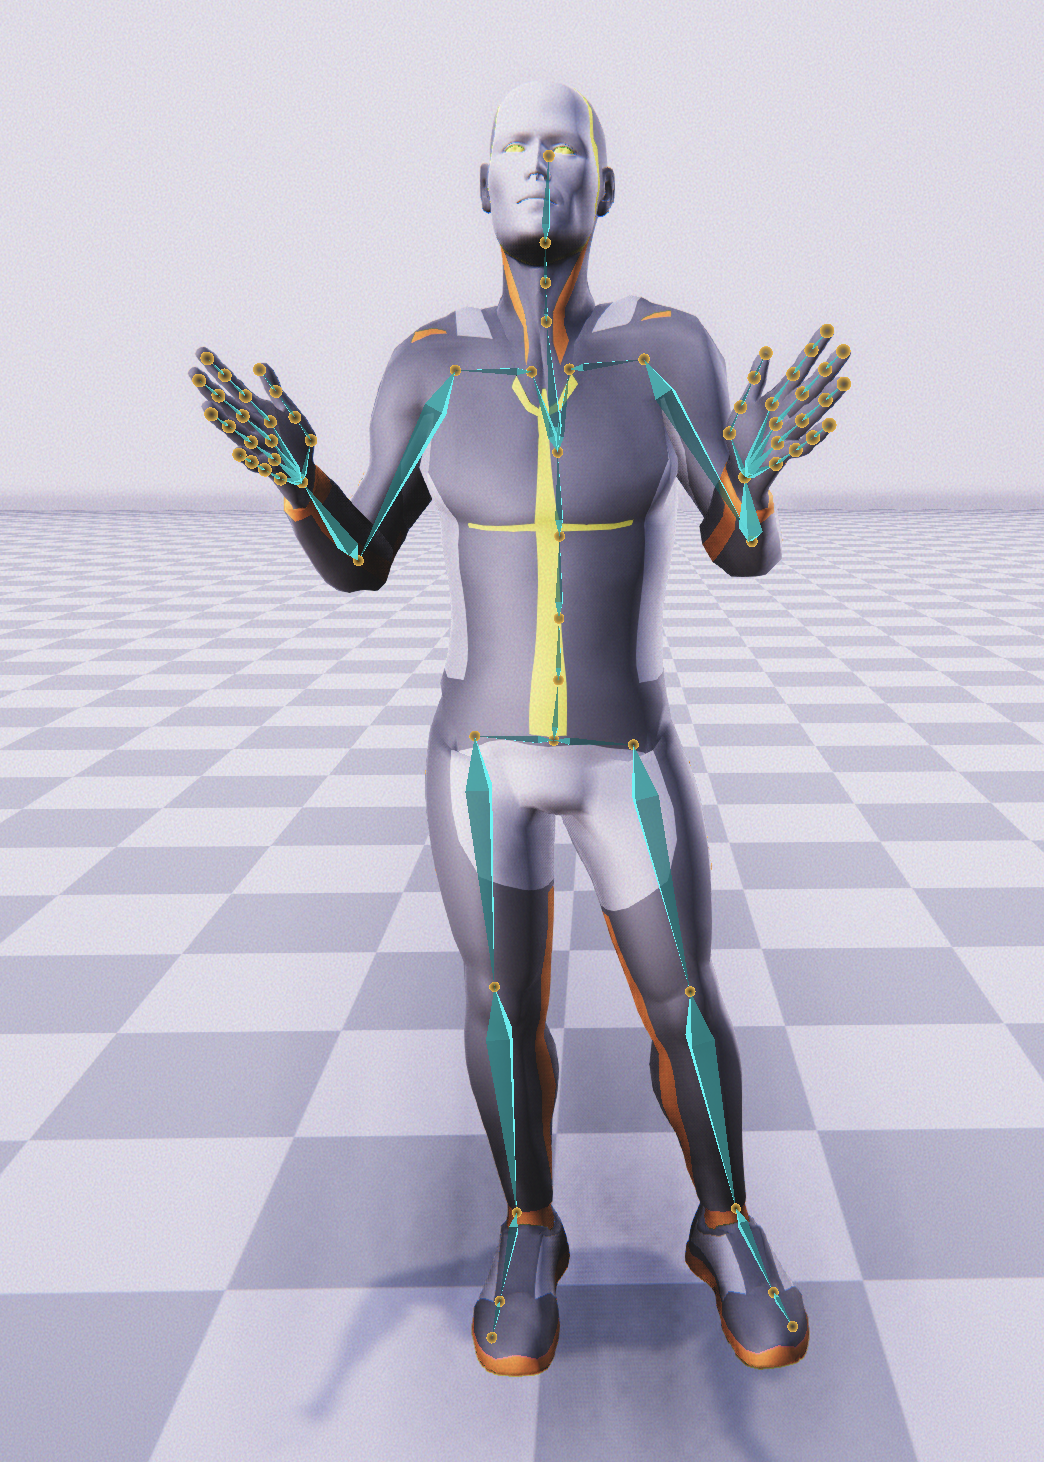
\includegraphics[height={6cm}]{SampleAnimation}
%	
%	\caption{Steven Job - Speech-Driven Gesture Generation}
%	\label{fig:SampleAnimation}
%
%\end{figure}
%
%\href{https://www.youtube.com/watch?v=B6nv1kQmi-Q}{\textcolor{blue}{\uline{youtube.com/watch?v=B6nv1kQmi-Q}}}

